\section{Minimal Kitaev Triangle}

We next show that the minimal Kitaev triangle suffices to demonstrate braiding of MZM. To this end we consider a closed path linearly interpolating between the following sets of values of $\phi_{jl}$:
\begin{align}
  (\phi_{12}, \phi_{23}, \phi_{31}) &= \left( 0, -\dfrac{\pi}{3}, -\dfrac{\pi}{3} \right) \equiv \bm\phi_1 \nonumber \\
  &\rightarrow \left( -\dfrac{\pi}{3}, -\dfrac{\pi}{3}, 0 \right) \equiv \bm\phi_2 \nonumber \\
  &\rightarrow \left( -\dfrac{\pi}{3}, 0, -\dfrac{\pi}{3} \right) \equiv \bm\phi_3 \nonumber \\
  &\rightarrow \bm\phi_1
\end{align}

It is straightforward to show that at $\bm \phi_{2}$ and $\bm \phi_3$ there are MZM located at sites $3,1$ and $2,3$, respectively.
Therefore the two original MZM at sites $1,2$ should switch their positions at the end of the adiabatic evolution.

\begin{figure}[ht]
  \centering
  \hspace{-25pt}
  \subfloat{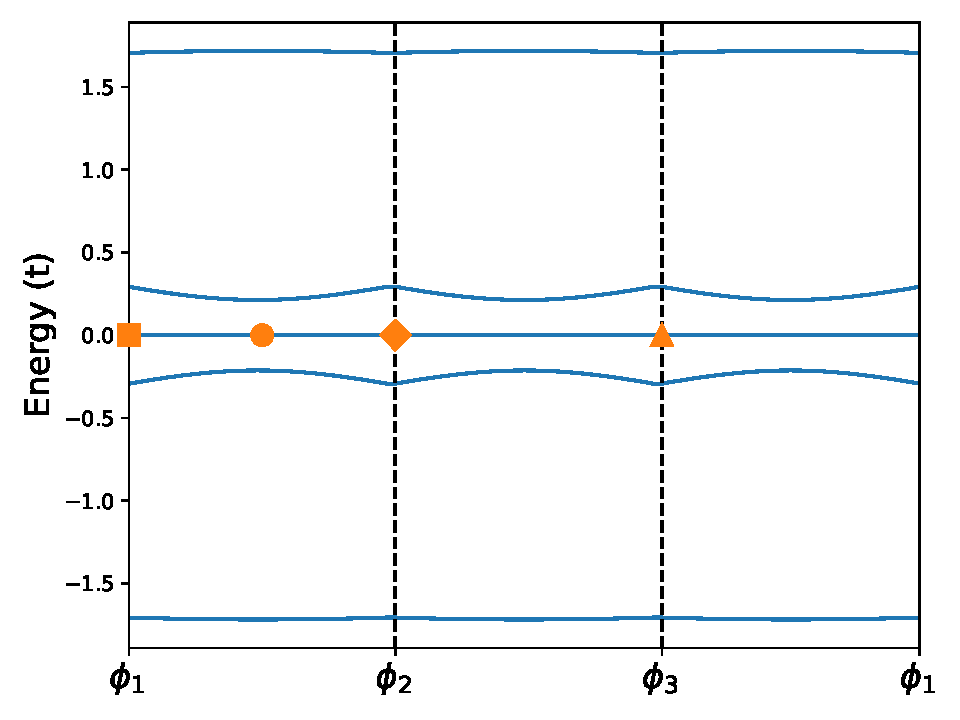
\includegraphics[width=0.5\textwidth]{3eigval.pdf}}\\
  \subfloat{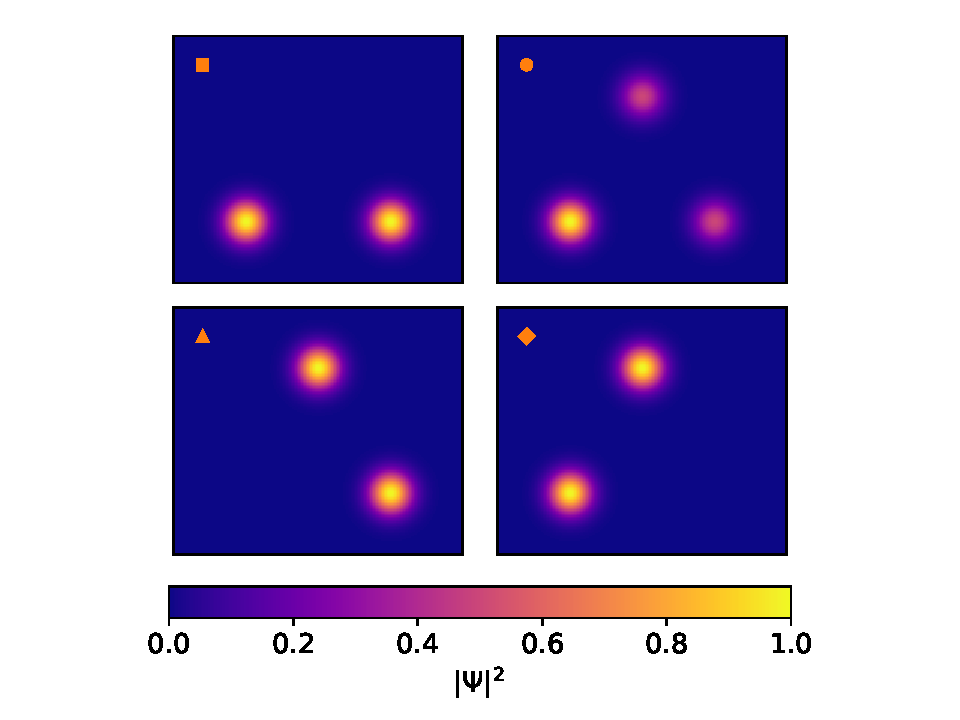
\includegraphics[width=0.6\textwidth]{3eigvec.pdf}}
  \caption{(a) Evolution of the eigenvalues of the 3-site Kitaev triangle along the closed parameter path for $\phi$ on the three edges. (b) MZM wavefunctions at different points of the parameter path. Clockwise from the upper left panel: $\bm \phi_1 \rightarrow \frac{1}{2}(\bm \phi_1 + \bm \phi_2)\rightarrow \bm \phi_2\rightarrow \bm\phi_3$.}
  \label{fig:3eig}
\end{figure}

Indeed, Fig.~\ref{fig:3eig} shows that the MZM stays at zero energy throughout the parameter path that interchanges their positions.
To show that such an operation indeed realizes braiding, we explicitly calculated the many-body Berry phase of the evolution and found the two degenerate many-body ground states acquire a $\frac{\pi}{2}$ difference in their Berry phases as expected.
Compared to the minimum T-junction model with four sites, our Kitaev triangle model only requires three sites to achieve braiding between two MZM, and is potentially also easier to engineer experimentally.
In the next section we will show that a more mesoscopic hollow-triangle structure can achieve similar results and may be preferred in other materials platforms.

